\documentclass[journal,12pt,twocolumn]{IEEEtran}
\usepackage[utf8]{inputenc}
\usepackage{kvmap}
\usepackage{graphics} 
\usepackage{setspace}
\usepackage{gensymb}
\singlespacing
\usepackage{amsthm}
\usepackage{mathrsfs}
\usepackage{txfonts}
\usepackage{stfloats}
\usepackage{bm}
\usepackage{cite}
\usepackage{cases}
\usepackage{subfig}

\usepackage{longtable}
\usepackage{multirow}

\usepackage{enumitem}
\usepackage{mathtools}
\usepackage{steinmetz}
\usepackage{tikz}
\usepackage{circuitikz}
\usepackage{verbatim}
\usepackage{tfrupee}
\usepackage[breaklinks=true]{hyperref}
\usepackage{graphicx}
\usepackage{tkz-euclide}
\usepackage{float}

\usetikzlibrary{calc,math}
\usepackage{listings}
    \usepackage{color}                                            %%
    \usepackage{array}                                            %%
    \usepackage{longtable}                                        %%
    \usepackage{calc}                                             %%
    \usepackage{multirow}                                         %%
    \usepackage{hhline}                                           %%
    \usepackage{ifthen}                                           %%
    \usepackage{lscape}     
\usepackage{multicol}
\usepackage{chngcntr}

\DeclareMathOperator*{\Res}{Res}

\renewcommand\thesection{\arabic{section}}
\renewcommand\thesubsection{\thesection.\arabic{subsection}}
\renewcommand\thesubsubsection{\thesubsection.\arabic{subsubsection}}

\renewcommand\thesectiondis{\arabic{section}}
\renewcommand\thesubsectiondis{\thesectiondis.\arabic{subsection}}
\renewcommand\thesubsubsectiondis{\thesubsectiondis.\arabic{subsubsection}}


\hyphenation{op-tical net-works semi-conduc-tor}
\def\inputGnumericTable{}                                 %%

\lstset{
%language=C,
frame=single, 
breaklines=true,
columns=fullflexible
}
\begin{document}


\newtheorem{theorem}{Theorem}[section]
\newtheorem{problem}{Problem}
\newtheorem{proposition}{Proposition}[section]
\newtheorem{lemma}{Lemma}[section]
\newtheorem{corollary}[theorem]{Corollary}
\newtheorem{example}{Example}[section]
\newtheorem{definition}[problem]{Definition}

\newcommand{\BEQA}{\begin{eqnarray}}
\newcommand{\EEQA}{\end{eqnarray}}
\newcommand{\define}{\stackrel{\triangle}{=}}
\newcommand\hlight[1]{\tikz[overlay, remember picture,baseline=-\the\dimexpr\fontdimen22\textfont2\relax]\node[rectangle,fill=blue!50,rounded corners,fill opacity = 0.2,draw,thick,text opacity =1] {$#1$};}
\bibliographystyle{IEEEtran}
\providecommand{\mbf}{\mathbf}
\providecommand{\pr}[1]{\ensuremath{\Pr\left(#1\right)}}
\providecommand{\qfunc}[1]{\ensuremath{Q\left(#1\right)}}
\providecommand{\sbrak}[1]{\ensuremath{{}\left[#1\right]}}
\providecommand{\lsbrak}[1]{\ensuremath{{}\left[#1\right.}}
\providecommand{\rsbrak}[1]{\ensuremath{{}\left.#1\right]}}
\providecommand{\brak}[1]{\ensuremath{\left(#1\right)}}
\providecommand{\lbrak}[1]{\ensuremath{\left(#1\right.}}
\providecommand{\rbrak}[1]{\ensuremath{\left.#1\right)}}
\providecommand{\cbrak}[1]{\ensuremath{\left\{#1\right\}}}
\providecommand{\lcbrak}[1]{\ensuremath{\left\{#1\right.}}
\providecommand{\rcbrak}[1]{\ensuremath{\left.#1\right\}}}
\theoremstyle{remark}
\newtheorem{rem}{Remark}
\newcommand{\sgn}{\mathop{\mathrm{sgn}}}
\providecommand{\abs}[1]{\left\vert#1\right\vert}
\providecommand{\res}[1]{\Res\displaylimits_{#1}} 
\providecommand{\norm}[1]{$\left\lVert#1\right\rVert$}
%\providecommand{\norm}[1]{\lVert#1\rVert}
\providecommand{\mtx}[1]{\mathbf{#1}}
\providecommand{\mean}[1]{E\left[ #1 \right]}
\providecommand{\fourier}{\overset{\mathcal{F}}{ \rightleftharpoons}}
%\providecommand{\hilbert}{\overset{\mathcal{H}}{ \rightleftharpoons}}
\providecommand{\system}{\overset{\mathcal{H}}{ \longleftrightarrow}}
	%\newcommand{\solution}[2]{\textbf{Solution:}{#1}}
\newcommand{\solution}{\noindent \textbf{Solution: }}
\newcommand{\cosec}{\,\text{cosec}\,}
\providecommand{\dec}[2]{\ensuremath{\overset{#1}{\underset{#2}{\gtrless}}}}
\newcommand{\myvec}[1]{\ensuremath{\begin{pmatrix}#1\end{pmatrix}}}
\newcommand{\mydet}[1]{\ensuremath{\begin{vmatrix}#1\end{vmatrix}}}
\renewcommand{\labelenumii}{\arabic{enumi}.\arabic{enumii}}
\renewcommand{\labelenumiii}{\arabic{enumi}.\arabic{enumii}.\arabic{enumiii}}
\renewcommand{\labelenumiv}{\arabic{enumi}.\arabic{enumii}.\arabic{enumiii}.\arabic{enumiv}}
\numberwithin{equation}{subsection}
\makeatletter
\@addtoreset{figure}{problem}
\makeatother
\let\StandardTheFigure\thefigure
\let\vec\mathbf
\renewcommand{\thefigure}{\theproblem}
\def\putbox#1#2#3{\makebox[0in][l]{\makebox[#1][l]{}\raisebox{\baselineskip}[0in][0in]{\raisebox{#2}[0in][0in]{#3}}}}
     \def\rightbox#1{\makebox[0in][r]{#1}}
     \def\centbox#1{\makebox[0in]{#1}}
     \def\topbox#1{\raisebox{-\baselineskip}[0in][0in]{#1}}
     \def\midbox#1{\raisebox{-0.5\baselineskip}[0in][0in]{#1}}
\vspace{3cm}

\title{ WIFI , BLUETOOTH WITH SEVEN SEGMENT UGV }

\author{S SRIKANTH REDDY}
\maketitle
\newpage
\bigskip
\renewcommand{\thefigure}{\theenumi}
\renewcommand{\thetable}{\theenumi}
\raggedright

%

\section*{Contents}
\begin{enumerate}
\item \textbf{Components} \hspace{4cm} 1\\
\item \textbf{Circuit Connections} \hspace{2.6cm} 1\\
\item \textbf{L293 Motor Driver} \hspace{2.7cm} 1\\
\item \textbf{WIFI Car Connections }\hspace{2.0cm} 1\\
\item \textbf{Seven Segment}\hspace{3.6cm} 1\\
\item \textbf{Working}\hspace{4.8cm} 1 \\
	\begin{enumerate}
	\item \textbf{Hardware Level}
	\item \textbf{Code}
	\end{enumerate}
\item \textbf{Execution} \hspace{4.45cm} 2 \\
\item \textbf{Execution For WIFI UGV} \hspace{1.4cm} 1 \\
\item \textbf{Components and Specifications} \hspace{0.5cm} 1 \\
\end{enumerate}
\section{Components}
\
\centering
\begin{tabular}{|l|c|c|}
\hline
Component & Value & Quantity\\
\hline
Vaman Board & & 1\\
\hline
USB-UART & & 1\\
\hline
UGV Chasis & & 1\\
\hline
DC Motors & & 2\\
\hline
Motor Driver Unit &  & 1\\
\hline
Jumper Wires & F-F & 10\\
\hline
Breadboard & & 1\\
\hline
\end{tabular}\\
\
\centerline{Table 1.0}

\section{Circuit Connections}
\raggedright
Make the Circuit Connections as per the table below.\\
\vspace{0.25cm}
\centering
\begin{tabular}{|c|c|}
\hline
Vaman Board & Motor Driver Unit\\
\hline
Pin 21 & Right Motor Input 1\\
\hline
Pin 18 & Right Motor Input 2\\
\hline
Pin 23 & Left Motor Input 1\\
\hline
Pin 22 & Left Motor Input 2\\
\hline
5V & VCC\\
\hline
GND & GND\\
\hline
\end{tabular}\\
\
\centerline{Table 2.0}
\section{L293 Motor Driver}
\raggedright
Make the Motor Driver Connections as per the table below.\\
\vspace{0.25cm}
\centering
\begin{tabular}{|c|c|c|c|}
\hline
INPUT & VAMAN BOAD &OUTPUT & MOTOR \\
\hline
A1 & PYGMY 21 & Vcc & 5V\\
\hline
A2 & PYGMY 18 & GND &GND  \\
\hline
EN & - & MA1 & MOTOR A1\\
\hline
VCC & 5V & MA2 & MOTOR A2\\
\hline
\hline
B2 & PYGMY 23 & MB1 & MOTOR B1\\
\hline
\hline
B1 & PYGMY 22 & MB2 & MOTOR B2\\
\hline
5V & VCC&-&-\\
\hline
GND & GND&-&-\\
\hline
\end{tabular}\\
\
\centerline{Table 3.0}
\section{WIFI CAR Connections}
\raggedright
Make the Circuit Connections as per the table below.\\
\vspace{0.25cm}
\centering
\begin{tabular}{|c|c|}
\hline
Vaman Board ESP 32 & Motor Driver Unit\\
\hline
Pin 16 & Right Motor Input 1\\
\hline
Pin 17 & Right Motor Input 2\\
\hline
Pin 18 & Left Motor Input 1\\
\hline
Pin 19 & Left Motor Input 2\\
\hline
5V & VCC\\
\hline
GND & GND\\
\hline
\end{tabular}\\
\
\centerline{Table 4.0}
\section{SevenSegment}
All codes used in this document are available at the following link.
\begin{lstlisting}
  https://github.com/gadepall/ugv/tree/main/codes/sevenseg
\end{lstlisting}

\section{Working}

\raggedright
\subsection{Hardware Level: }

On the hardware level there are three key points: SPI, Wishbone Interfacing and Address Mapping.\\
\vspace{0.2cm}

On the Vaman Board, we have an EOS S3 and ESP32. The Communication between these two happens via SPI i.e, \textbf{Serial Peripheral Interface}. And this is facilitated only when all the 4 jumpers on the board are closed. \\

\vspace{0.25cm}

The EOS S3 has an ARM M4 Core, a FPGA unit and 512 KB of SRAM along with a AHB. The SRAM is divided into 4 banks. Banks 0-2 are accessible only by the ARM M4. Bank 3 is accessible by any master connected to \textbf{Always-ON Bus}. FPGA a slave on that AON Bus. \\
The same can be observed from the figure below.\\

\vspace{0.5cm}
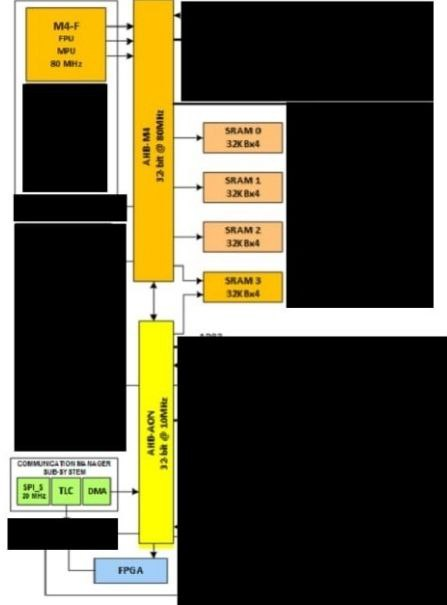
\includegraphics[width=0.5\textwidth]{eos.jpg}
\centerline{Figure 1 - EOS S3 Architecture}
\

Now, the communication between ARM M4 Core and the FPGA unit takes place via the AHB Bus. For this to happen, we implement \textbf{Wishbone slave interface} on the FPGA. Without this Wishbone slave interface the communication with FPGA registers is not possible. The master requests from the ARM4 Core on the AHB are converted to wishbone signals and hence reach FPGA. \\
\vspace{0.25cm}

\includegraphics[width=0.5\textwidth]{wishbone.jpg}
\centerline{Figure 2 - Wishbone Slave Interface}
\

And the next key thing is to know the starting address of the FPGA Registers in EOS S3 Memory organisation (which is provided by the manufacturer). Hence, mapping them to read or write the FPGA Registers. 

\raggedright
\subsection{Code: }

In the code also there are three major processes that take place in ESP32, ARM Core and FPGA.\\
\vspace{0.25cm}

Firstly, The ESP32 collects the joystick movement data from the Dabble app connected via bluetooth. It receives the x,y co-ordinates in the range [-7,7]. EP32 then scales it to [0,255] and places it in the Arrays declared in the ARM Core. \\

\vspace{0.25cm}

The ARM Core now has the joystick movement data in its 8 bit registers. Which it passes on to the mapped FPGA Registers via the AHB.\\

\vspace{0.25cm}

Then in FPGA we implement the Wishbone slave interface to read the data sent by the ARM Core via AHB. Now in the FPGA Unit, the Pulse Width Modulation takes place. The corresponding PWM values for the joystick movement data are generated and sent back to the ARM Core.\\

\vspace{0.25cm}

Now the ARM Core running a loop, Checks if the Cross or Square button is pressed and also reads these changes in the PWM values. It then sends signal to the DC Motors of the UGV to rotate the wheels accordingly.\\

\section{Execution}
\raggedright
1. Download the repository

\begin{lstlisting}
svn co https://github.com/srikanth9515/FWC/tree/main/UGV
\end{lstlisting}

2. Build the ESP32 firmware
\begin{lstlisting}
cd esp32_pwmctrl
pio run
\end{lstlisting} 

3. Flash ESP32 firmware ( connect USB-UART adapter )
\begin{lstlisting}
pio run -t nobuild -t upload
\end{lstlisting} 

4. If using termux, send .pio/build/esp32doit-devkit-v1/firmware.bin to PC using
\begin{lstlisting}
scp .pio/build/esp32doit-devkit-v1/firmware.bin Username@IPAddress:
\end{lstlisting} 

5.  Modify line 140 of config.mk to setup path to pygmy-sdk and then Build m4 firmware using
\begin{lstlisting}
cd m4_pwmctrl/GCC_Project
make
\end{lstlisting}

6. If using termux, send output/m4{\_}pwmctrl.bin to PC using
\begin{lstlisting}
scp output/m4_pwmctrl.bin username@IPaddress:
\end{lstlisting} 

7. Build fpga source (.bin file)
\begin{lstlisting}
cd fpga_pwmctrl/rtl
ql_symbiflow -compile -d ql-eos-s3 -P pu64 -v *.v -t AL4S3B_FPGA_Top -p quickfeather.pcf -dump jlink binary 
\end{lstlisting} 

8. If using termux, send AL4S3B{\_}FPGA{\_}Top.bin to PC using
\begin{lstlisting}
scp AL4S3B_FPGA_Top.bin username@IPaddress:
\end{lstlisting} 

9. Connect usb cable to vaman board and Flash eos s3 soc, using
\begin{lstlisting}
sudo python3 <Type path to tiny fpga programmer application> --port /dev/ttyACM0  --appfpga AL4S3B_FPGA_Top.bin --m4app m4_pwmctrl.bin --mode m4-fpga --reset
\end{lstlisting} 

10. Install the \textbf{Dabble app} on the Mobile from the \textbf{Playstore}. Connect it to the \textbf{ESP32} on the Vaman Board using \textbf{Bluetooth}. Change the controls to \textbf{Joystick mode} to navigate the UGV.\\

\section{Execution For WIFI UGV}
\raggedright
1. Download the repository
\begin{lstlisting}
https://github.com/srikanth9515/FWC/tree/main/WIFI_UGV
\end{lstlisting}

2. Build the ESP32 firmware
\begin{lstlisting}
cd esp32_pwmctrl
pio run
\end{lstlisting} 

3. Flash ESP32 firmware ( connect USB-UART adapter )
\begin{lstlisting}
pio run -t upload
\end{lstlisting} 

4. Connect your own TAB /Phone Hot spot and  Enter Your SSID &  Password
\begin{lstlisting}
const char* ssid = "srikanth";         /*Enter Your SSID*/ 
const char* password = "srikanth123"; /*Enter Your Password*
\end{lstlisting} 
5. Install the \textbf{APK app} on the Mobile from the \textbf{Playstore}. Connect it to the \textbf{ESP32} on the Vaman Board using \textbf{Wifi}. Change the controls to \textbf{Joystick mode} to navigate the UGV.\\

\section{Components and Specifications}
\includegraphics[width=0.5\textwidth]{ugv gallery.png}
\centerline{Figure 3 - DC motors}

\includegraphics[width=0.5\textwidth]{ugv gallery.png}
\centerline{Figure 4 - UGV frame/chassis}

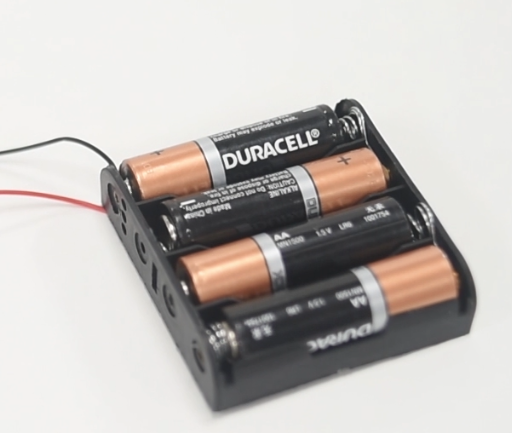
\includegraphics[width=0.5\textwidth]{battery.png}
\centerline{Figure 5 - Batteries}
Assemble the Chassis using the provided nuts/screws, Wheels, and parts
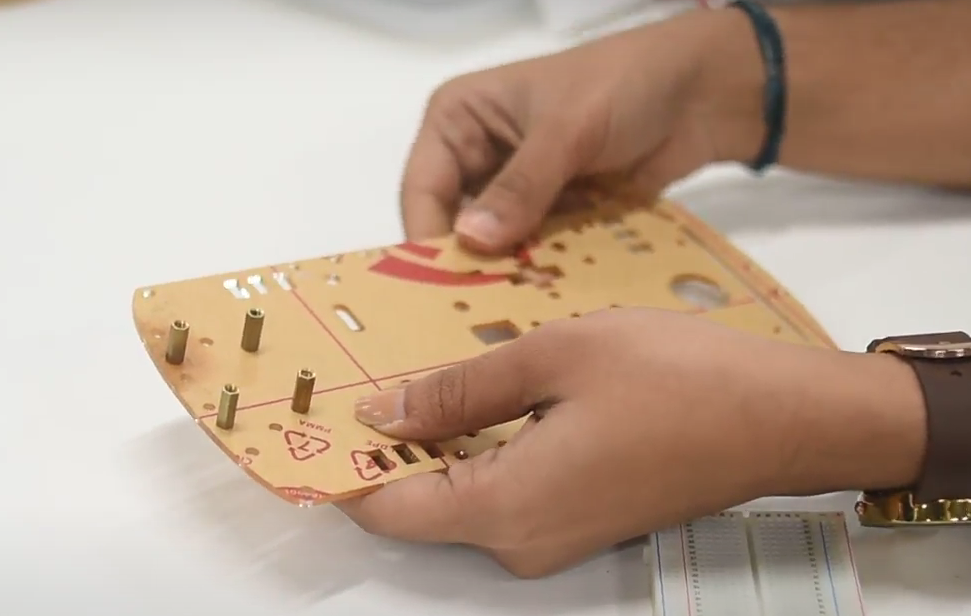
\includegraphics[width=0.5\textwidth]{f1.png}
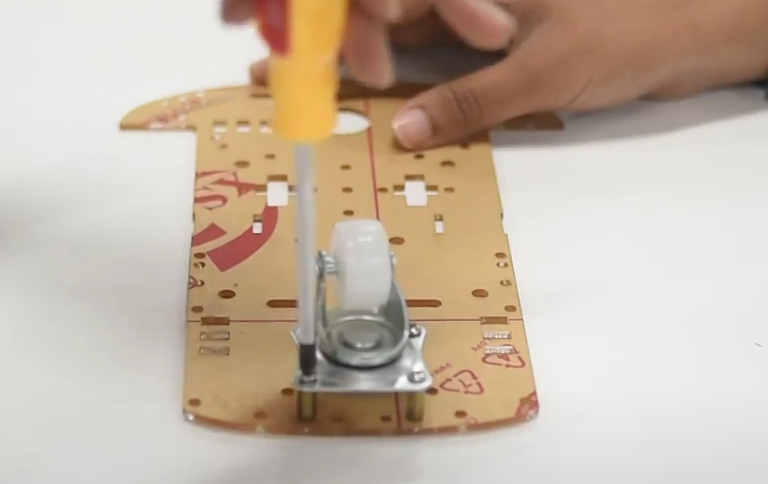
\includegraphics[width=0.5\textwidth]{f2.png}
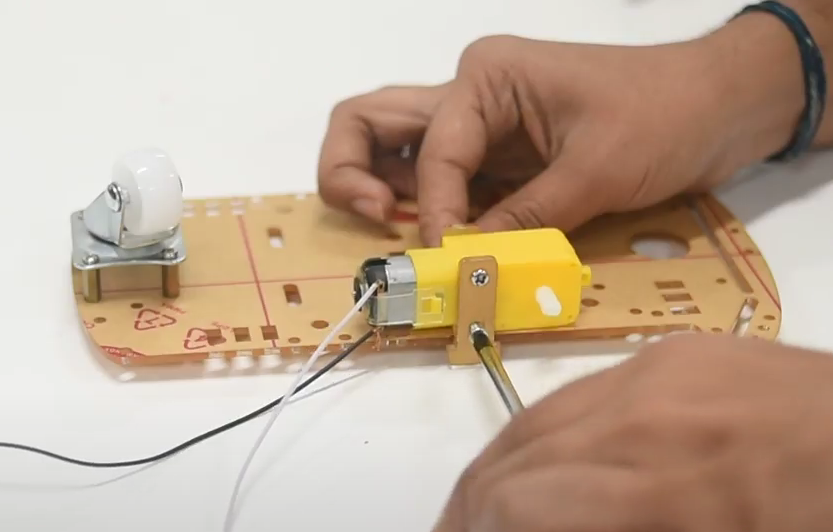
\includegraphics[width=0.5\textwidth]{f3.png}
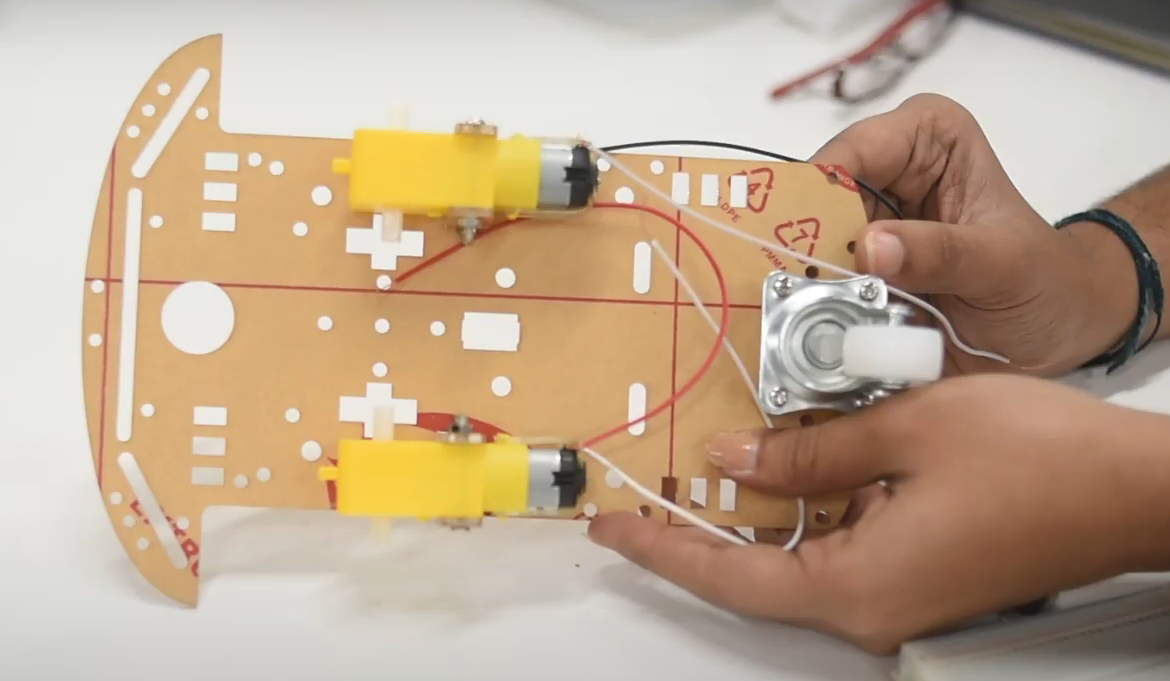
\includegraphics[width=0.5\textwidth]{f5.png}
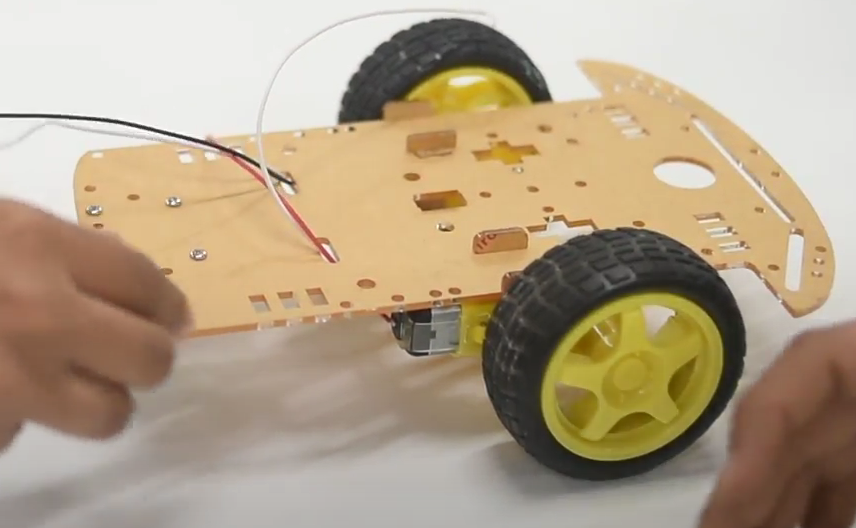
\includegraphics[width=0.5\textwidth]{f6.png}
\centerline{Figure 6 - Assembling the UGV kit}
◦ Fix the Vaman controller and ESP32 on the chassis.
◦ Fix the Dual motor driver IC along with a small breadboard on the chassis.
◦ Fix the Li-Po battery on the chassis and insert AA batteries in the battery holder.

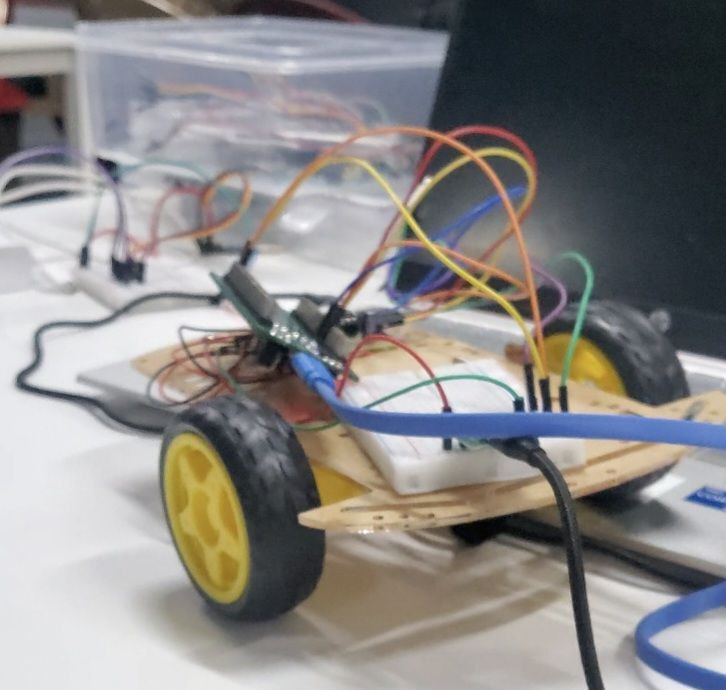
\includegraphics[width=0.5\textwidth]{car.jpg}
\centerline{Figure 7 -  Connections UGV }
Connect the battery supply and turn on the power to various equipment.
◦ Download the “dabble” application from the play store on an Android phone.
◦ Using dabble application, connect to the ESP32 on the UGV kit using Bluetooth connection.
◦ Control the navigation of the UGV kit using the GUI controls on the dabble application.


\section{Seven Segment Display Output For WIFI}
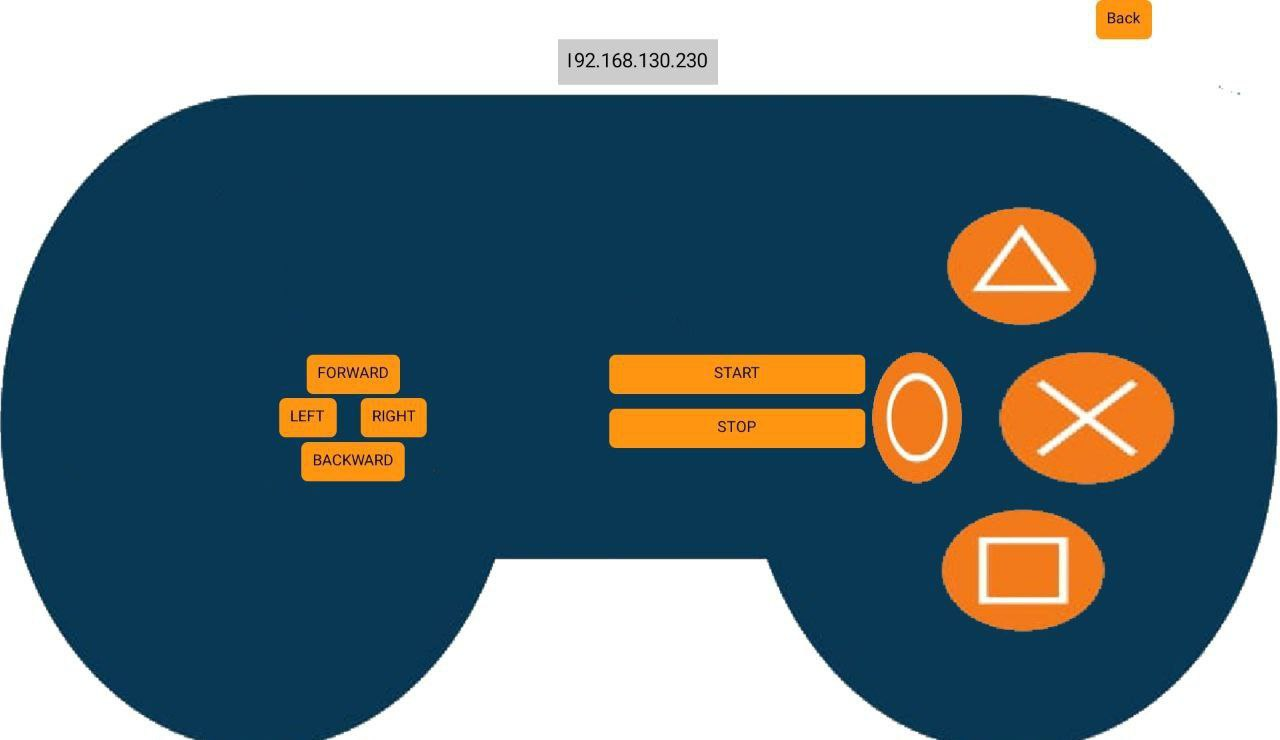
\includegraphics[width=0.5\textwidth]{remote.jpg}
\centerline{Figure 8 -   Seven segment Display with UGV }
\includegraphics[width=0.5\textwidth]{zero.jpg}
\centerline{Figure 9 -   Stop Will Display zero }
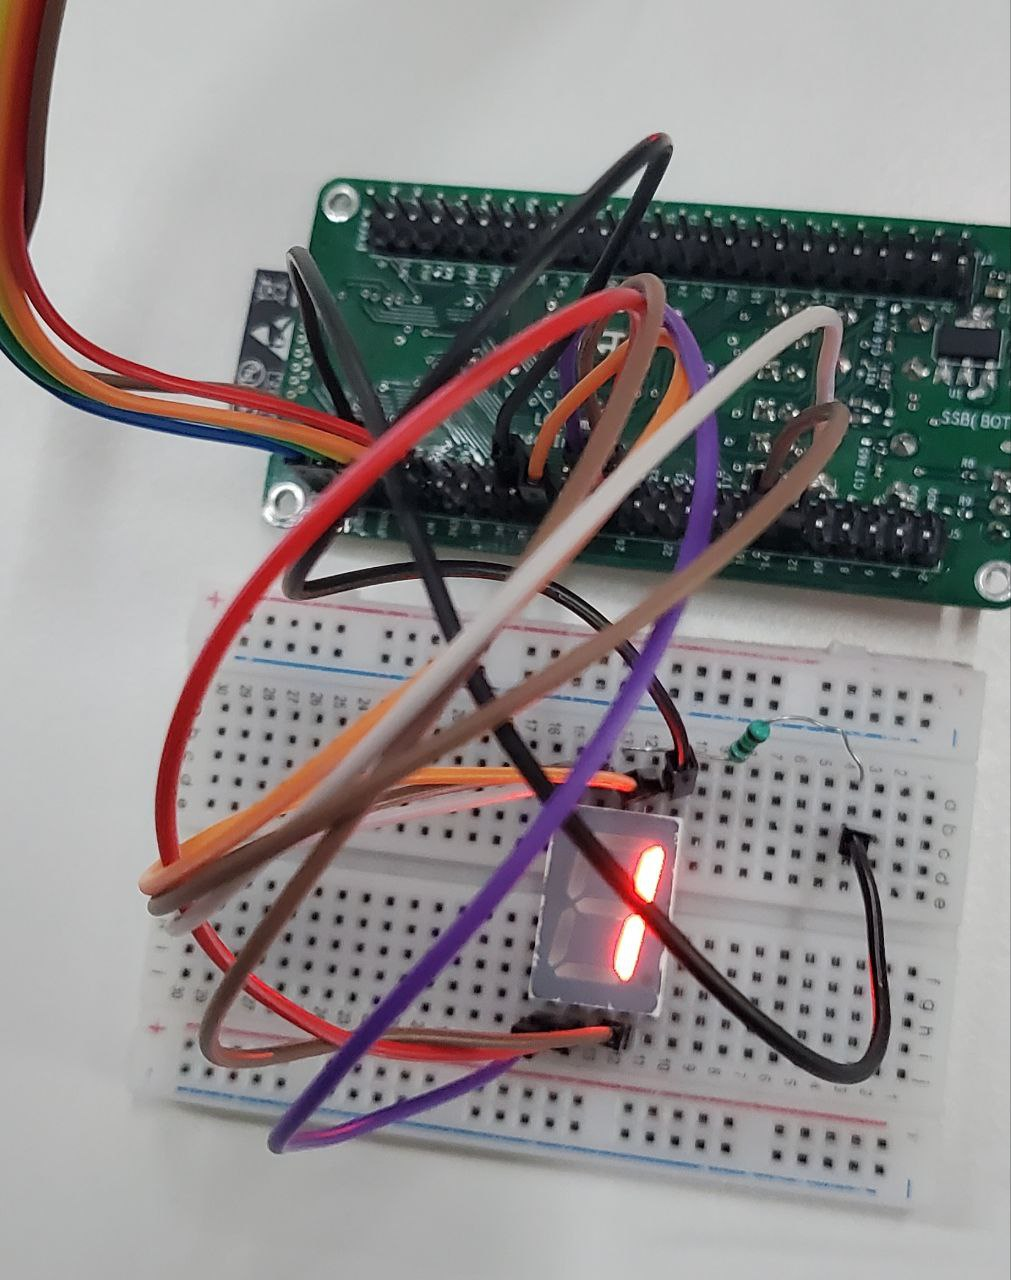
\includegraphics[width=0.5\textwidth]{one.jpg}
\centerline{Figure 10 -  Start Will Display One }
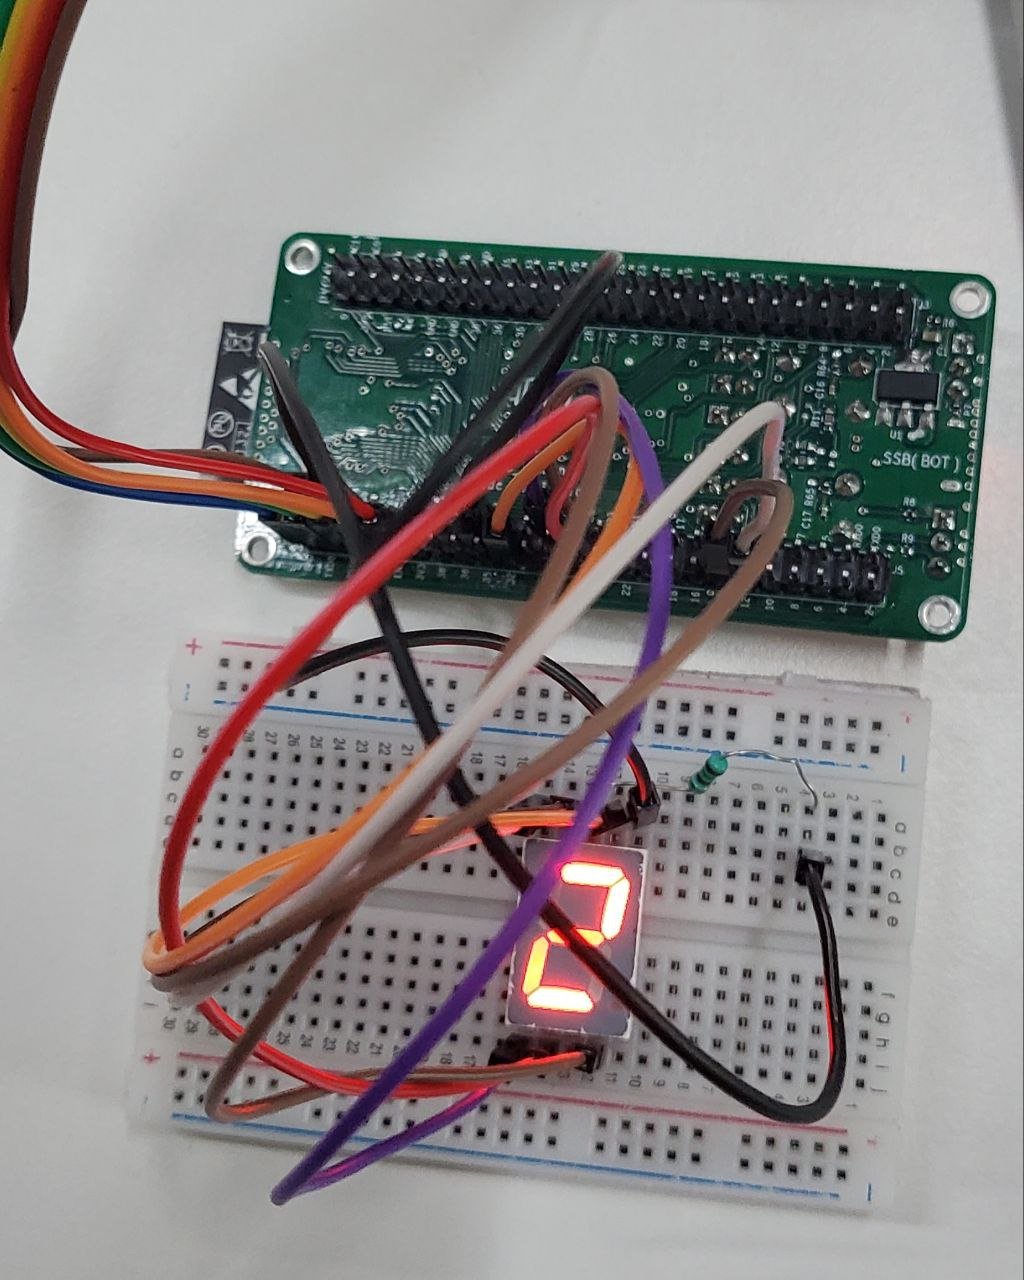
\includegraphics[width=0.5\textwidth]{two.jpg}
\centerline{Figure 11 -  Forward Will Display Two }
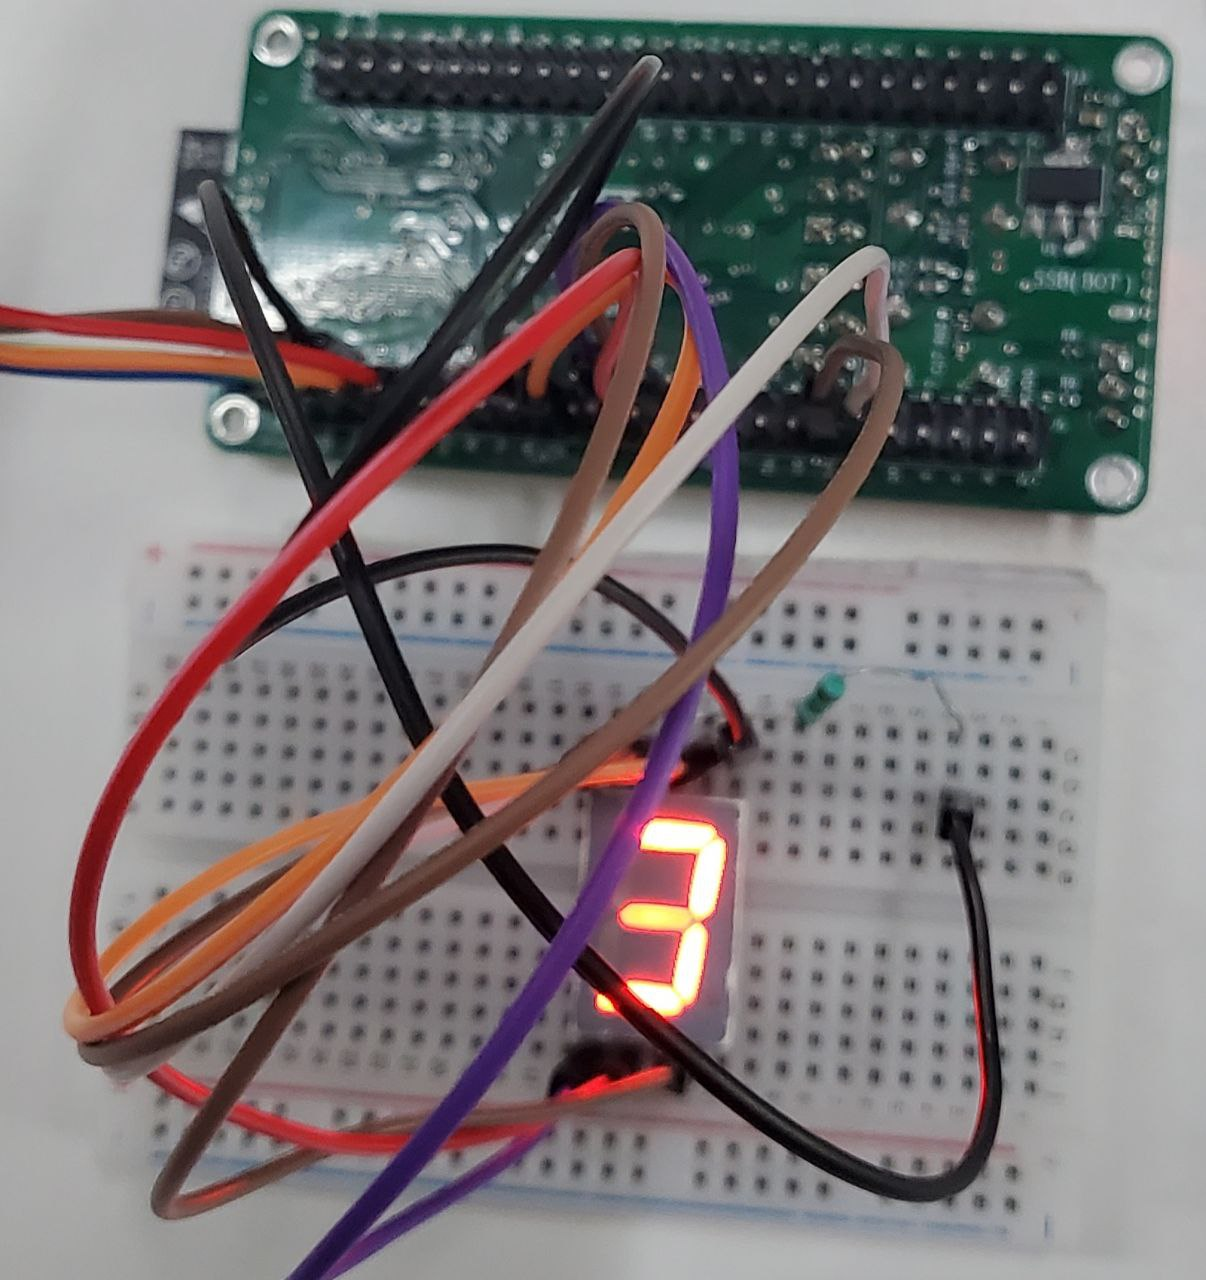
\includegraphics[width=0.5\textwidth]{three.jpg}
\centerline{Figure 12 -  Back ward Will Display Three }
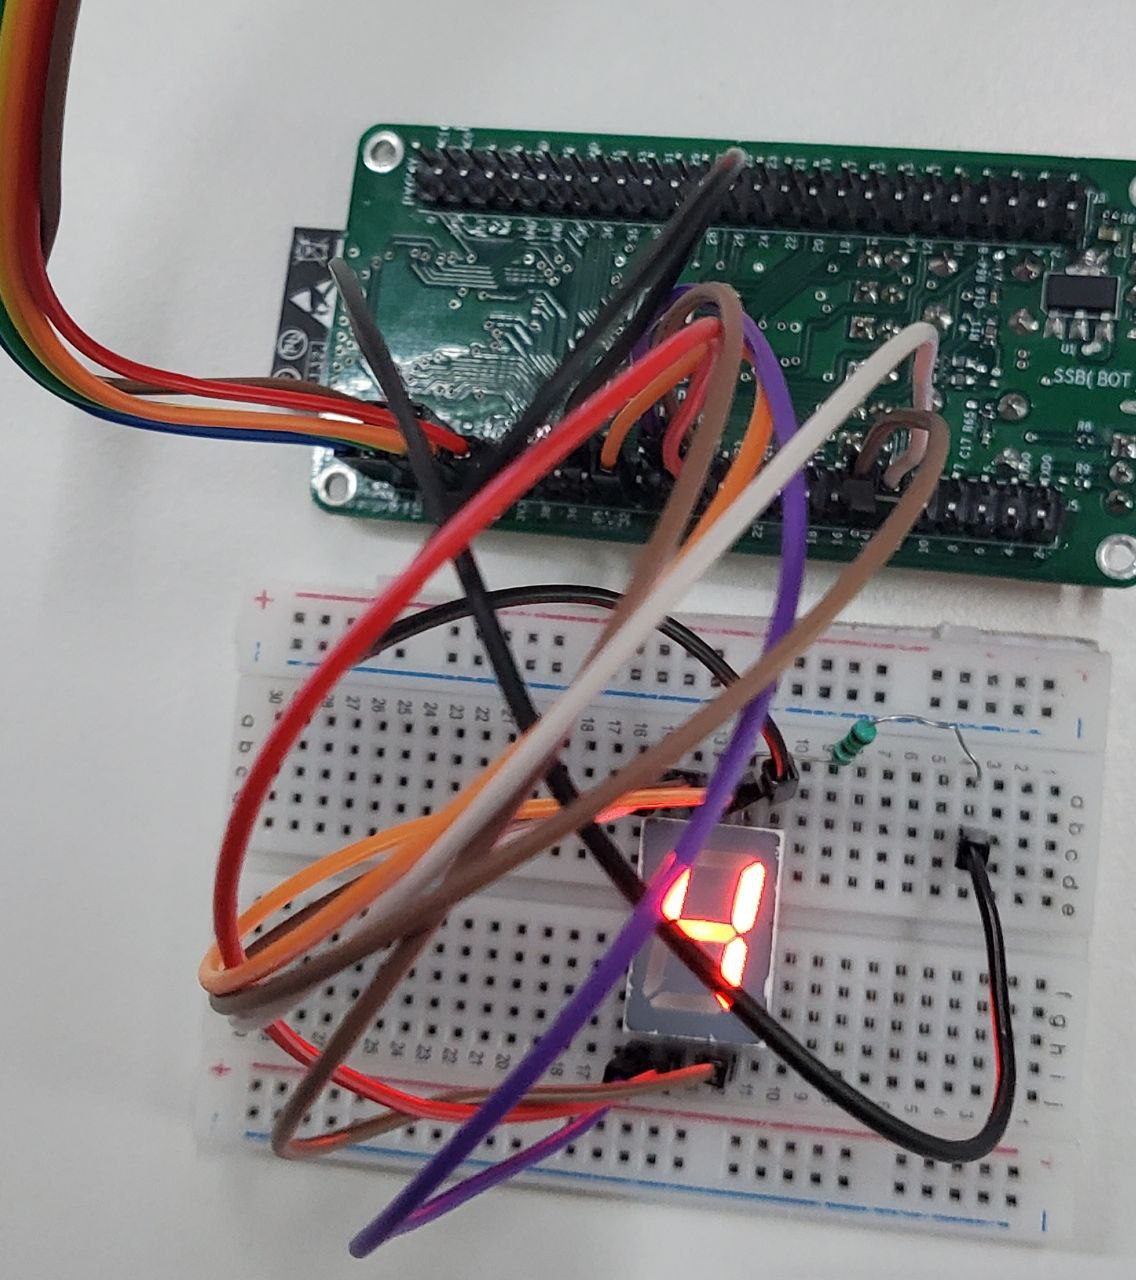
\includegraphics[width=0.5\textwidth]{four.jpg}
\centerline{Figure 13 -  Left Will Display Four }
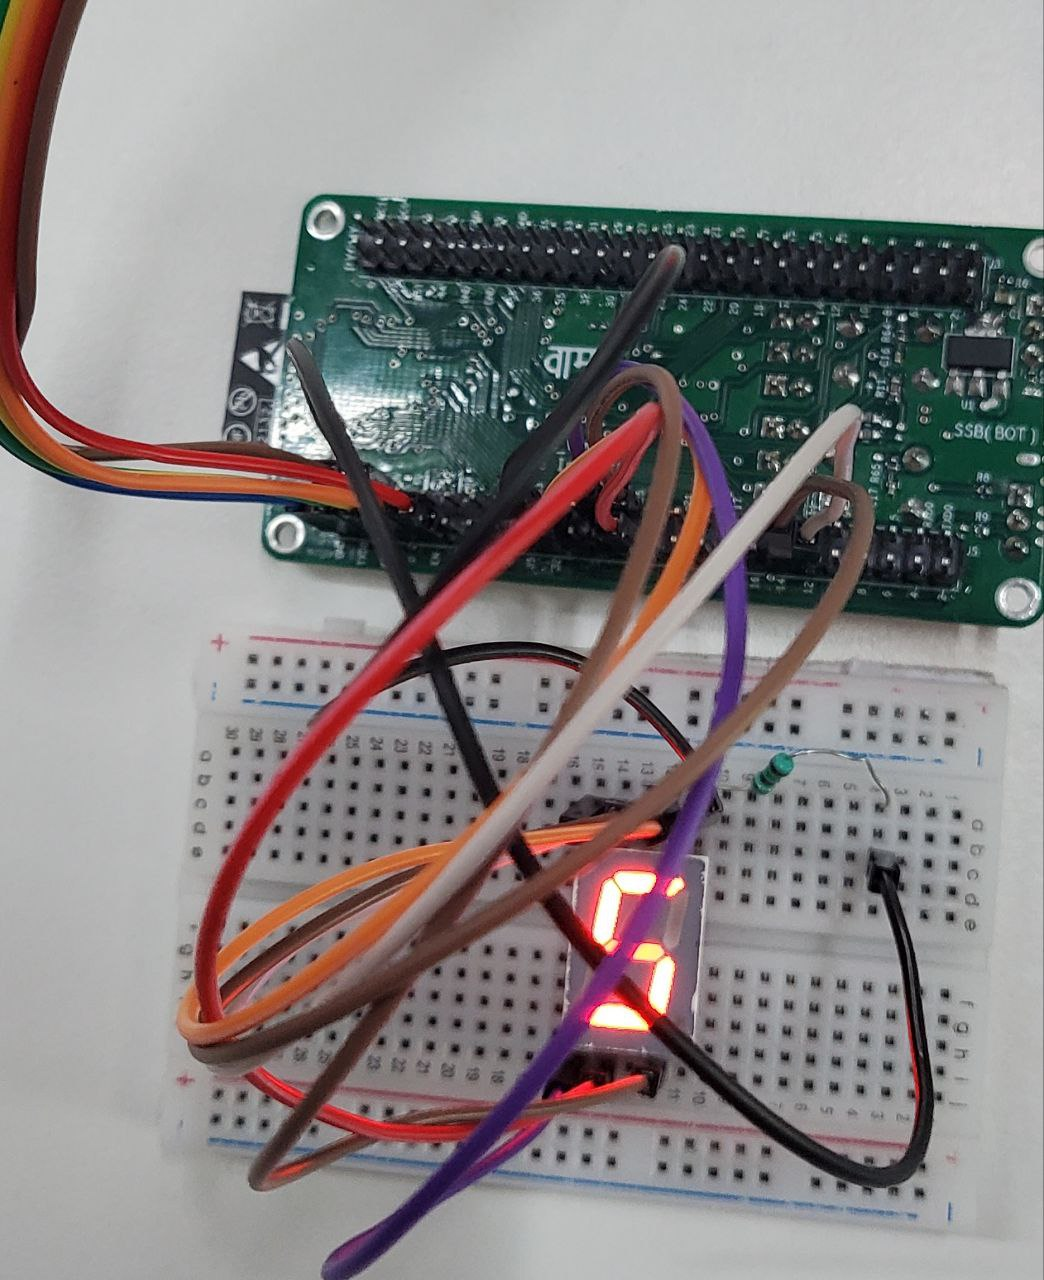
\includegraphics[width=0.5\textwidth]{five.jpg}
\centerline{Figure 14 -  Right Will Display Five }
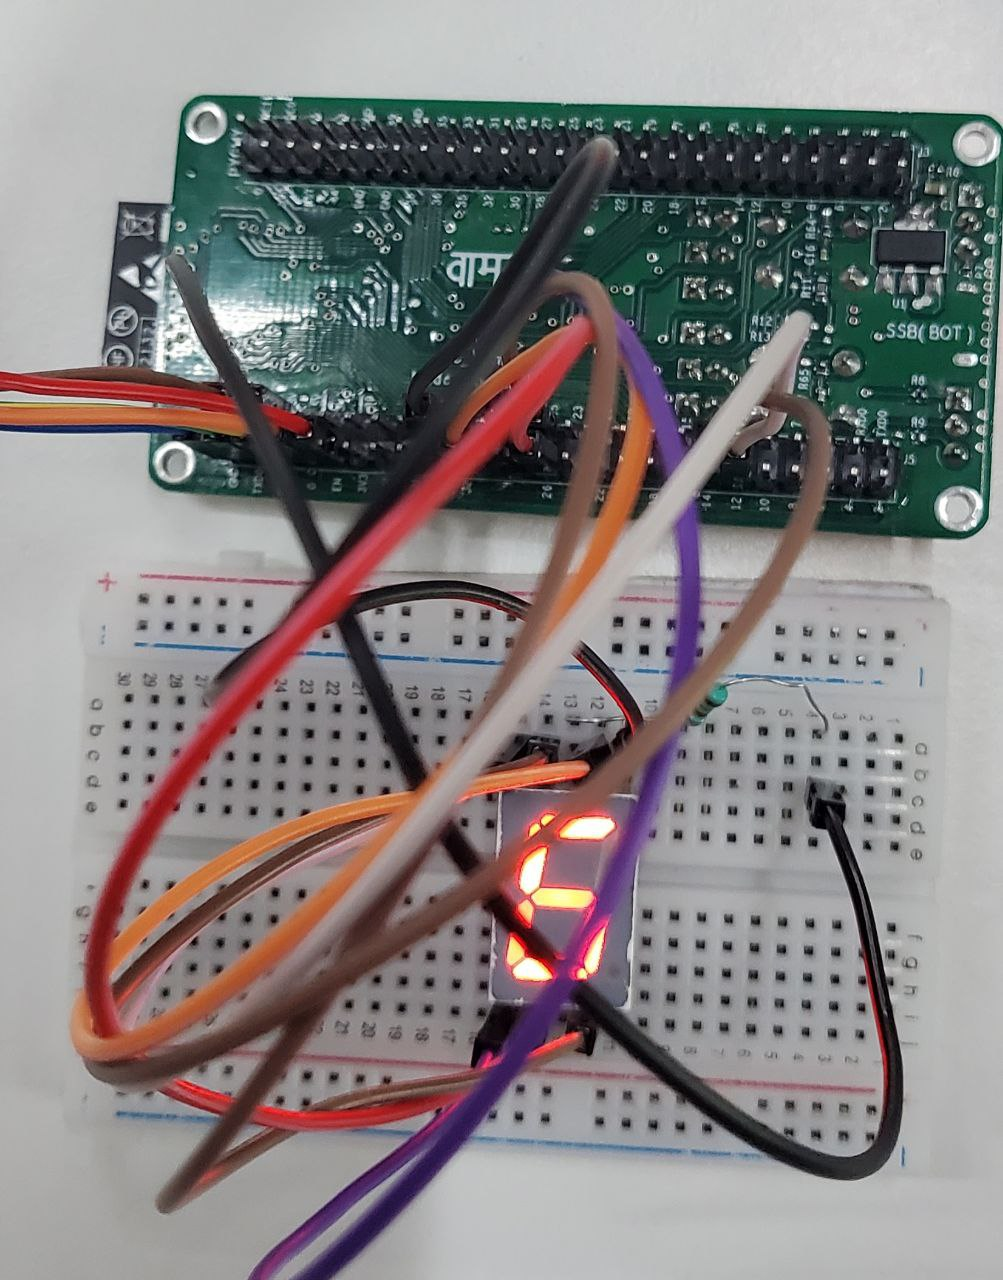
\includegraphics[width=0.5\textwidth]{six.jpg}
\centerline{Figure 15 -  Cross Will Display Six }
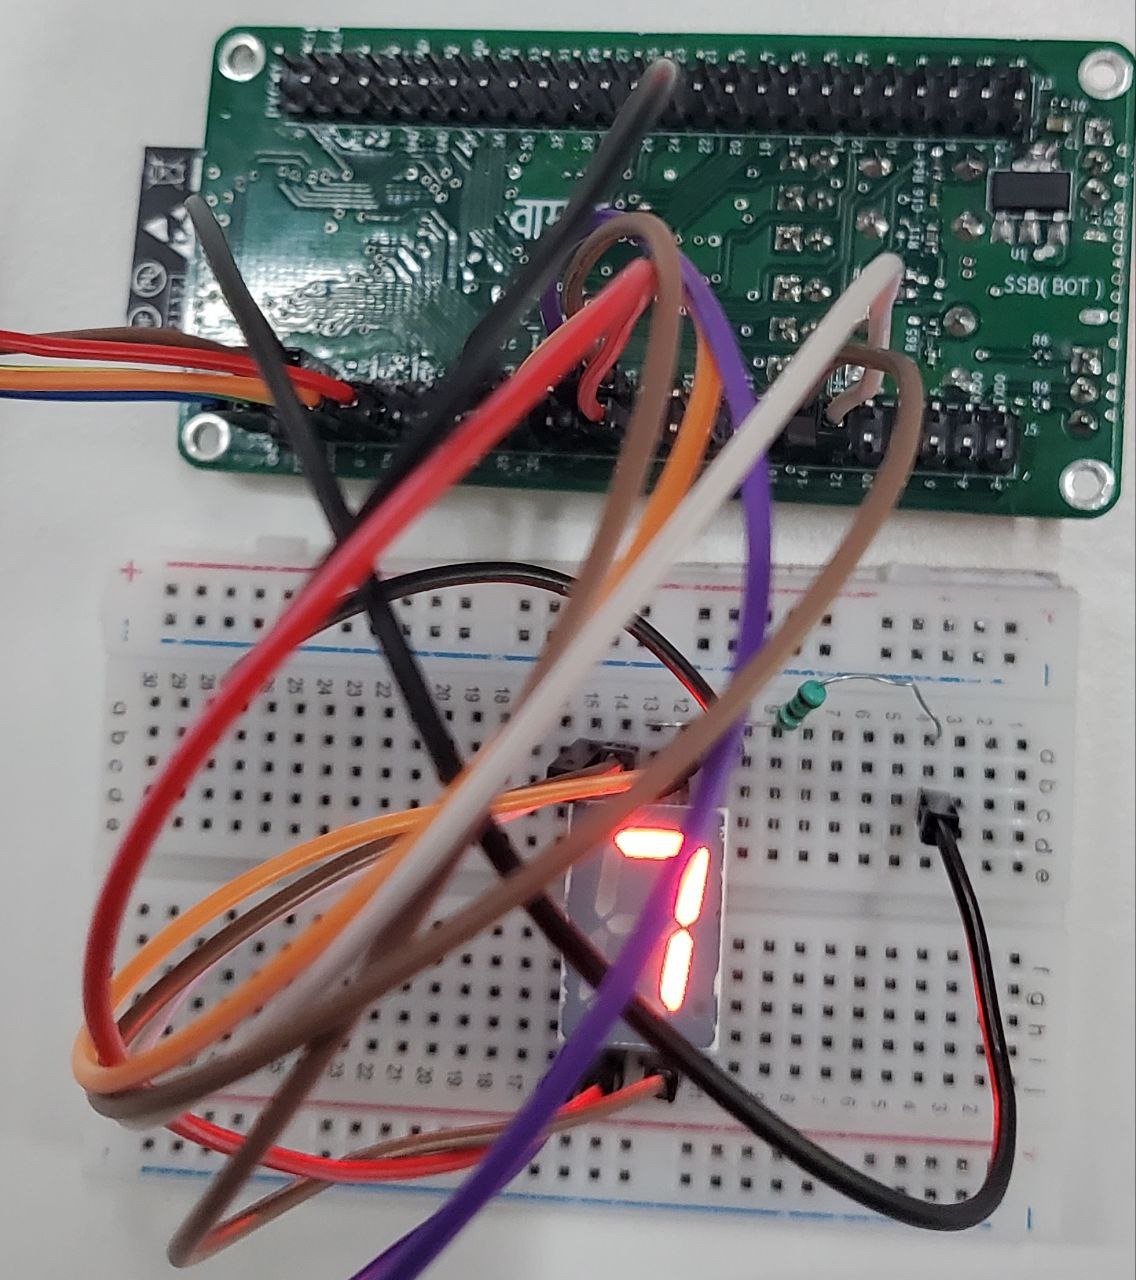
\includegraphics[width=0.5\textwidth]{seven.jpg}
\centerline{Figure 16 -  Circle Will Display Seven }
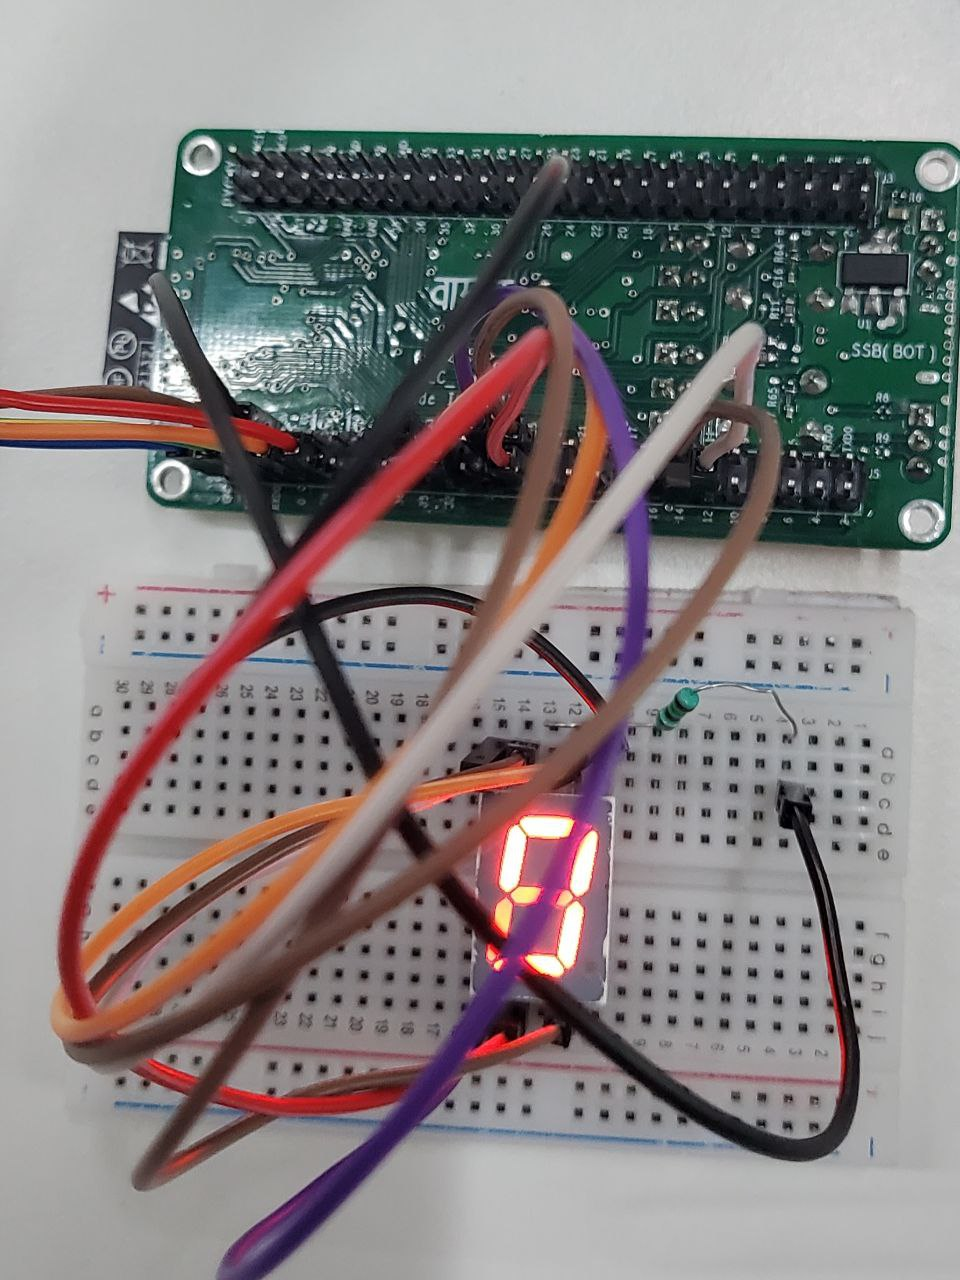
\includegraphics[width=0.5\textwidth]{eight.jpg}
\centerline{Figure 17 -  React Angle Will Display Eight }
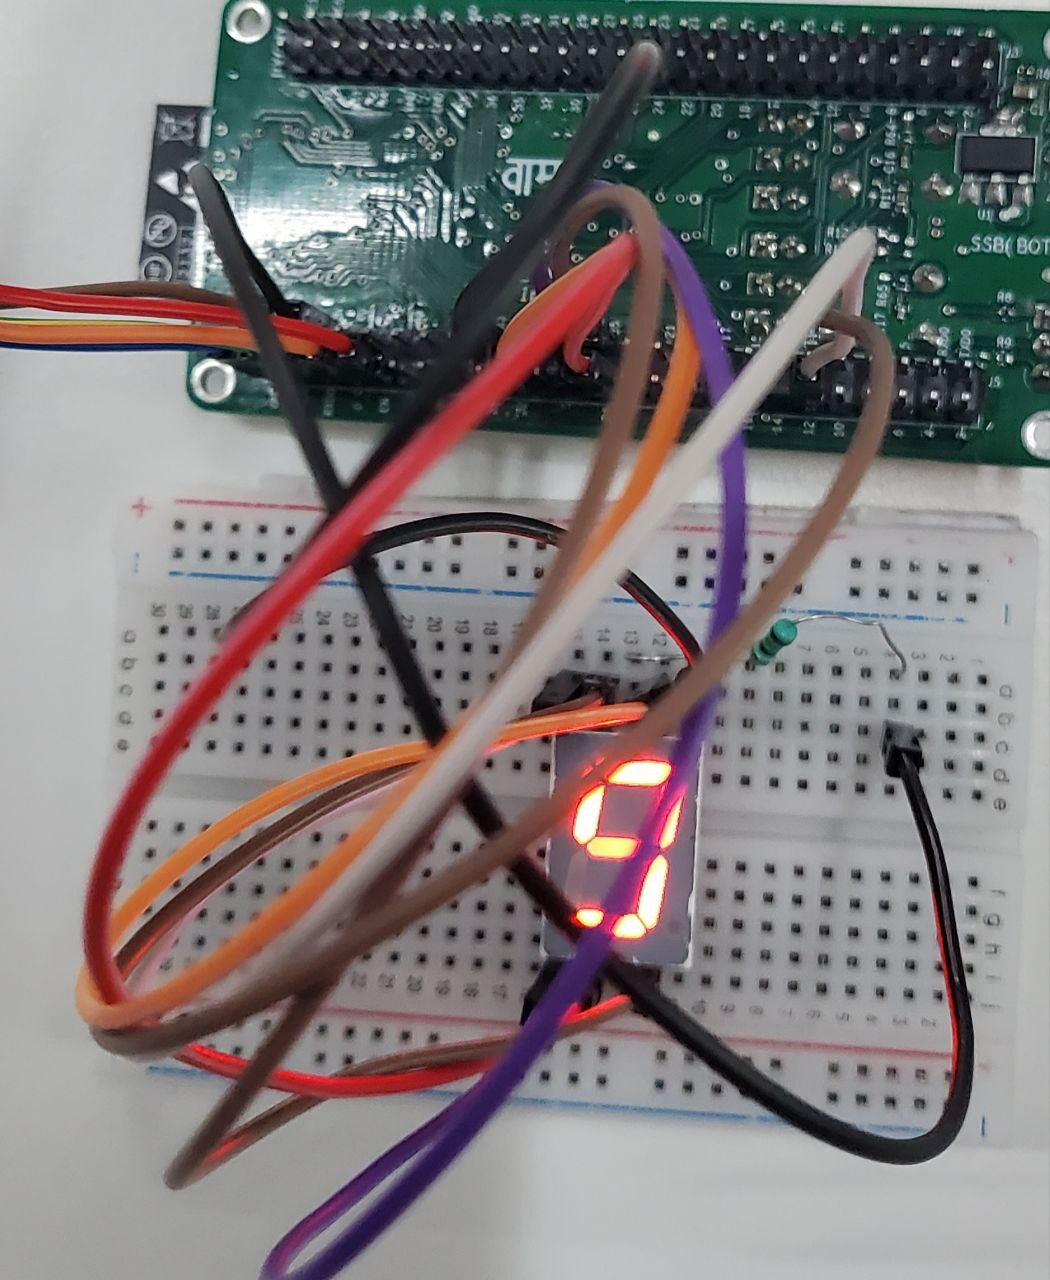
\includegraphics[width=0.5\textwidth]{nine.jpg}
\centerline{Figure 10 -  Triangle Will Display Nine }

\end{document}



